\documentclass[english,handout]{beamer}
%\documentclass[english]{beamer} 
\usepackage{amsmath}
\usepackage{graphicx}

%\makeatletter
\input xy
\xyoption{all}


\usepackage{listings}
\usepackage{hyperref}
\usetheme{Boadilla}

\setbeamercovered{transparent}

\usecolortheme{purdue}

\usepackage{babel}


\title[Consensus]{Consensus Among Computer Networks}

\author{Darren Tapp}
\institute[ASU]
{
  Arizona State University
}
\date{November 18, 2020}

\begin{document}


\begin{frame}
  \titlepage
\end{frame}


\begin{frame}
\frametitle{Consensus}

Academic organization:
\begin{itemize}
\item<2->
Byzantine Fault Tolerance
\item<3->
Nakamoto Consensus
\item<4->
Dash Consensus

\end{itemize}

\end{frame}

\begin{frame}
\frametitle{Citations}

\begin{itemize}
\item<1-> BFT: Several peer reviewed articles, e.g. \\
\href{https://blog.tappmath.com/files/Practical_Byzantine_Fault_Tolerance.pdf}{``Practical Byzantine Fault Tolerance''}
\item<2-> Nakamoto Consensus: \href{https://blog.tappmath.com/files/bitcoin.pdf}{``Bitcoin: A Peer-to-Peer Electronic Cash System''}
\item<3-> Dash Consensus: \href{https://github.com/dashpay/dips}{Dash Improvement Proposals 2,3,6-8}
\end{itemize}

\end{frame}

\begin{frame}
\frametitle{Byzantine Fault Tolerance}

For an open network
\begin{block}{Byzantine Fault Tolerance }
\begin{itemize}
\item Is vulnerable to Sybil attacks
\item Fails (generally) if over one third of nodes are malicious
\item Requires multiple communication rounds
\end{itemize}
\end{block}
\end{frame}

\begin{frame}
\frametitle{Nakamoto Consensus}

For an open network
\begin{block}{Nakamoto Consensus }
\begin{itemize}
\item Mitigates Sybil attacks with proof of work
\item Can be verified by a passive node
\item Generally runs at a stable Nash equilibrium
\end{itemize}
\end{block}

\end{frame}

\begin{frame}
\frametitle{Nakamoto Consensus}

\[
\xymatrix{
\cdots \ar[r] &*+[F]{\textrm{Block 5}} \ar[r] &*+[F]{\textrm{Block 6}} \ar[r] & \cdots
}
\]
\vspace{0.5 in}
\pause

\begin{center}
The consensus is about a global state (UTXO) and the blocks are instructions for
changing the global state (transactions.)
\end{center}


\end{frame}

\begin{frame}
\frametitle{Nakamoto Consensus}
A Nakamoto network could be out of consensus
\pause
\[
\xymatrix{ &  &*+[F]{\textrm{Block 7}} \\
\cdots \ar[r]& *+[F]{\textrm{Block 6}} \ar[ur] \ar[dr] \\
 & &*+[F]{\textrm{Block 7'}} }
\]
\pause
This diagram shows a blockchain where the most recent changes could be in dispute.

\pause
Consensus is still maintained over old changes.

\end{frame}


\begin{frame}
\frametitle{Nakamoto Consensus}

However, the network will collapse into a consensus by following \\
the longest chain
\pause
\[
\xymatrix{ & &*+[F]{\textrm{Block 7}} \\
\cdots \ar[r] & *+[F]{\textrm{Block 6}} \ar[ur] \ar[dr] \\
  & &*+[F]{\textrm{Block 7'}} \ar[r] &*+[F]{\textrm{Block 8}}
}
\]

\end{frame}

\begin{frame}
\frametitle{Dash Consensus}

Outline:

The remaining portion of this seminar will be for \\
explaining existing Dash consensus implementations

\begin{itemize}
\item<2-> Quick overview of what a Dash consensus is
\item<3-> Choice of threshold signature scheme
\item<4-> Byzantine Resistance; ``Quorum Math''
\item<5-> Applications of ChainLocks and InstantSend
\end{itemize}

\end{frame}

\begin{frame}
\frametitle{What is Dash Consensus?}

A Dash consensus requires a blockchain to provide Nakamoto consensus.

\begin{enumerate}
\item<2> Register actors on chain with public key
\item<3> Select subset, called a quorum, of registered actors
\item<4> Produce threshold signature of statement/datum that is in consensus
\end{enumerate}

\end{frame}

\begin{frame}
\frametitle{Nomenclature}

\begin{center}
If $M$ actors are registered and a subset on $n$ actors is selected and a
threshold of $t$ out of the $n$ actors is required for signature.
\end{center}
We call this a:

\[
\textrm{Dash}(M,n,t) \textrm{ Consensus}
\]

for security reasons we assume $t>\frac{n}{2}$.\\
We also assume that the quorum of n nodes is a simple
random sample of the M registered.\\
In practice, a simple random selection is simulated using hash functions.


\end{frame}

\begin{frame}
\frametitle{Register on Chain}

\begin{center}
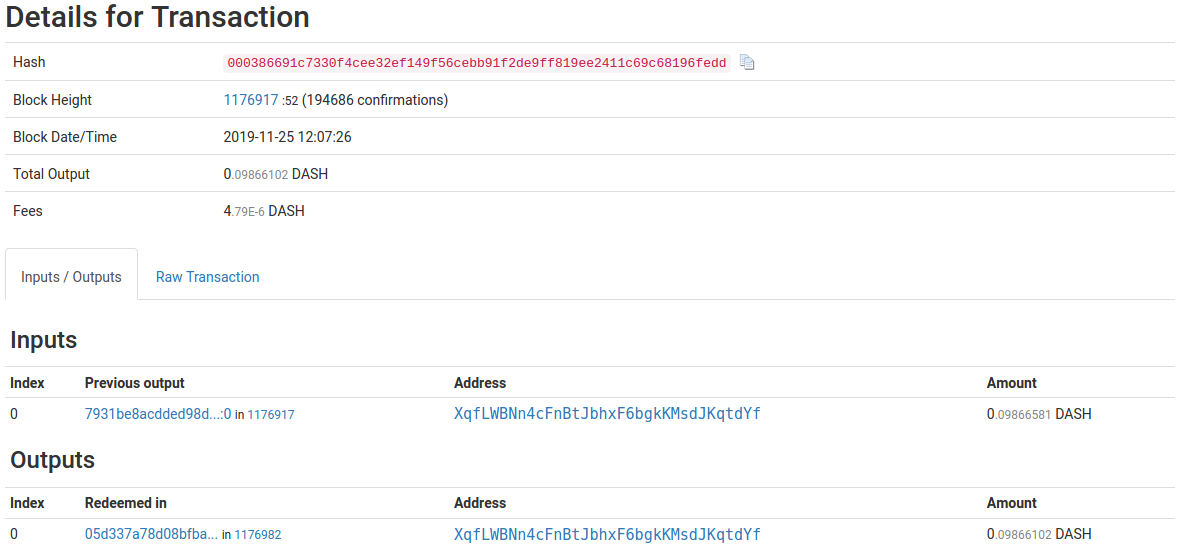
\includegraphics[width=4in]{Reg_tx.png}
\end{center}

\end{frame}

\begin{frame}
\frametitle{Register on Chain}

\begin{center}
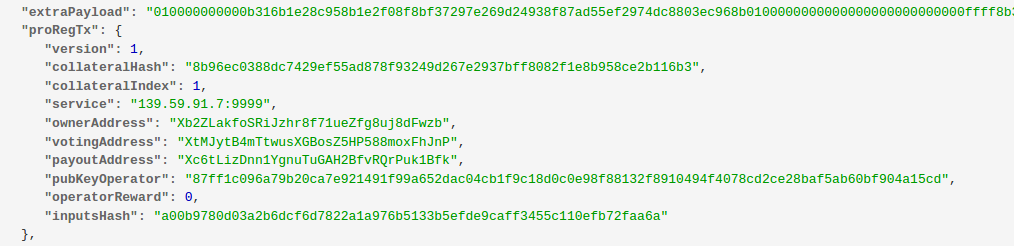
\includegraphics[width=4in]{extra_payload.png}
\end{center}
\pause
collateralHash and collateralIndex point out 1000 dash on chain.\\
\pause
This 1000 dash requirement mitigates a Sybil attack. \\
\pause
ownerAddress, voterAddress, and payoutAddress are base 58 encoding of ECDSA keys.\\
\pause
pubKeyOperator is a hexadecimal encoding of a BLS public key. \\
\pause
This key is what's used for Dash consensus.
\end{frame}

\begin{frame}
\frametitle{Choice of Threshold Signature}

We'll compare two threshold signature schemes:

\begin{itemize}
\item Schnorr signatures
\item BLS signatures
\end{itemize}
\end{frame}

\begin{frame}
\frametitle{Na\"ive Multisignature}
\vfill
For Schnorr and BLS signature schemes, \\
public keys are points on elliptic curves.
\pause
\vfill
If three actors publish their public keys $P$,$Q$ and $R$ \\
a multisignature is a valid signature for $P+Q+R$.
\vfill

\end{frame}

\begin{frame}
\frametitle{Related-key Attack}

Alice Bob and Malory want to construct an multisignature.  \\
\pause
\begin{itemize}
\item Alice obtains private key $a$ with public key $A$ and publishes $A$
\item Bob obtains private key $b$ with public key $B$ and publishes $B$
\pause
\item Malory obtains private key $c$ with public key $C$ \\
but publishes $C-A-B$
\end{itemize}
\pause
Then an aggregate signature will be for the key
\[
A+B+C-A-B = C.
\]
\pause
Since Malory knows the corresponding private key of C \\
he can construct an aggregate signature without Alice or Bob.
\end{frame}

\begin{frame}
\frametitle{Advantages}
\vfill
\begin{center}
Schnorr signatures can work with ECDSA keys that are \\currently used for Dash payments.
\end{center}
\pause
\vfill
\begin{center}
BLS signatures are easier to construct on the fly and \\
they have a smaller attack surface.
\end{center}
\vfill
\end{frame}

\begin{frame}
\frametitle{Long Story Short}
\vfill
\begin{center}
Schnorr signatures require each party to provide entropy.\\
This entropy is combined before a signature can be constructed. \\
If something goes wrong in the entropy stage  \\
then the process must start over.  \\
{\bf Reusing entropy could allow private keys to be solved for.}
\end{center}
\vfill
\begin{center}
BLS signatures do not require entropy.
\end{center}
\vfill
\end{frame}

\begin{frame}
\frametitle{Citation}
\begin{center}
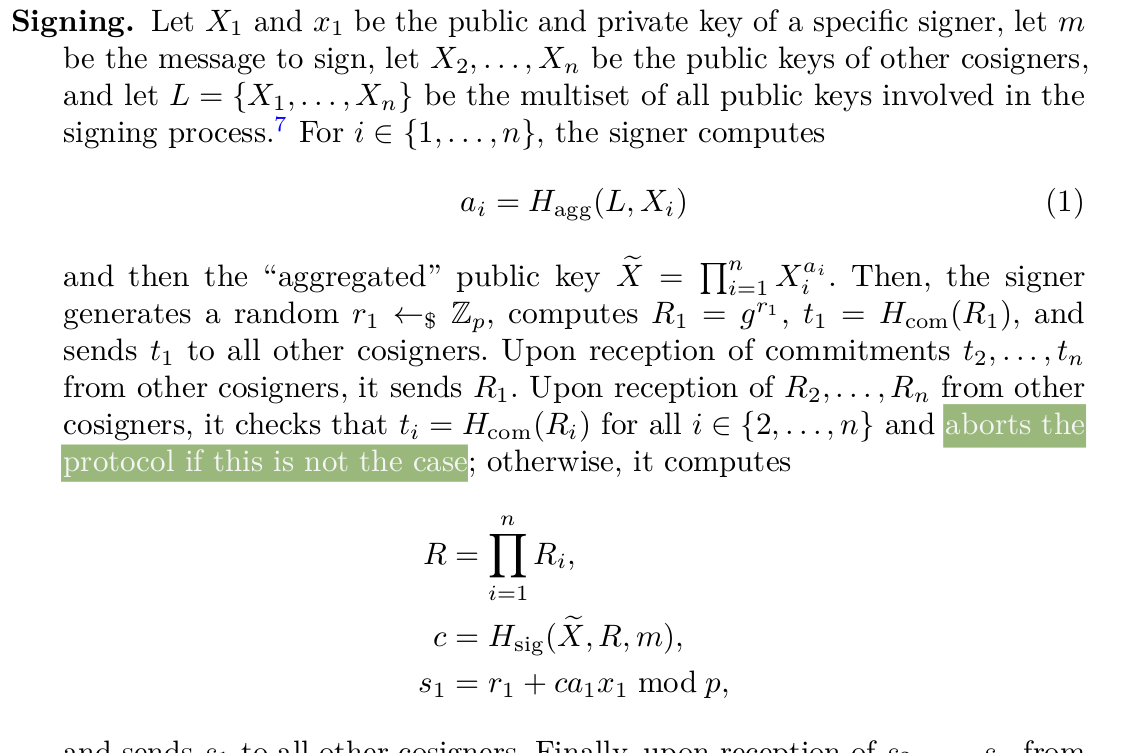
\includegraphics[width=3.5in]{aborts.png}
\end{center}

\href{https://eprint.iacr.org/2018/068.pdf}{Cite page 11 of:\\
``Simple Schnorr Multi-Signatures with Applications to Bitcoin''}

\end{frame}

\begin{frame}
\frametitle{Citation}
\begin{center}
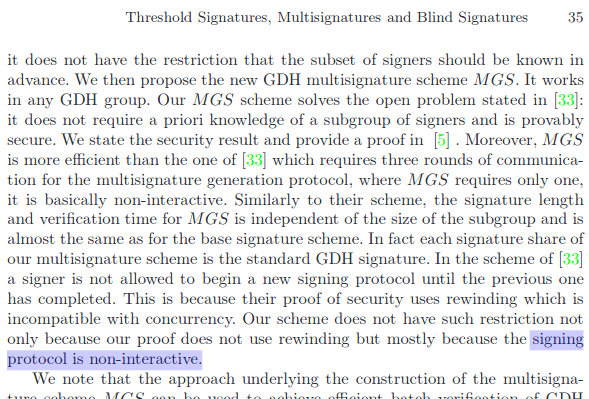
\includegraphics[width=3.2in]{non-interactive.png}
\end{center}

\href{https://blog.tappmath.com/files/Boldyreva2002.pdf}{Cite page 35 of: \\``Threshold Signatures, Multisignatures and Blind Signatures Based on the Gap-Diffie-Hellman-Group Signature Scheme''}

\end{frame}

\begin{frame}
\frametitle{Clarification}

\begin{center}
A BLS threshold signature, has an interactive \\ Distributed Key Generation phase. \\
\vspace{10pt}
After that, all threshold signatures are non-interactive.

For a $t$ out of $n$ threshold signature.  Any party with $>t$
signature shares can create a valid threshold signature.
\end{center}
\end{frame}

\begin{frame}
\frametitle{Byzantine Resistance}


A Byzantine actor attempts to disrupt or alter $\textrm{DASH}(M,n,t)$ consensus by registering or
controlling nodes.  \\
There are two types of attacks that a Byzantine actor can employ.

\vfill

\begin{block}{Byzantine DOS}
The actor has control of and/or has disabled $> n-t$ nodes to prevent a signature from being formed
\end{block}
\vfill

\begin{block}{Byzantine Hijack}
The actor controls $\geq t$ nodes and can produce any signature.
\end{block}


\end{frame}

\begin{frame}
\frametitle{Byzantine Resistance}

When considering a $\textrm{DASH}(M,n,t)$ consensus. There are $M$ choose $n$
possible quorums that can be selected. Recall that $M$ choose $n$ is a binomial
coefficient and written
\[
{M \choose n}
\]
If $b$ out of the $M$ nodes are Byzantine, and $b>t$ then there are
\[
{M-b \choose n-t}{b \choose t}
\]
quorums that contain exactly $t$ Byzantine nodes. So the probability that a quorum
has more than t Byzantine nodes is
\[
\frac{\sum_{j=t}^{\textrm{max}(n,b)} {M-b \choose n-j}{b \choose j}}{{M \choose n}}
\]

\end{frame}


\begin{frame}
\frametitle{Byzantine Resistance}
For a $\textrm{DASH}(5000,400,240)$ consensus.\\

\begin{center}
\begin{tabular}{|c|c|c|c|}
\hline
Byzantine & Byzantine & DOS  & Hijack \\
Proportion & Nodes & probability & probability\\
\hline
$0.05$ & $250$ & 4.19e-125& 1.27e-284\\
\hline
$0.10$ & $500$ & 3.31e-65& 7.11e-157\\
\hline
$0.20$ & $1000$ & 1.68e-22& 2.89e-76\\
\hline
$0.30$ & $1500$ & 3.37e-06& 1.29e-38\\
\hline
$0.34$ & $1700$ & 3.81e-3 & 1.23e-28\\
\hline
$0.40$ & $2000$ & 0.478& 3.21e-17\\
\hline
$0.50$ & $2500$ & 0.99999& 1.82e-05 \\
\hline
\end{tabular}
\end{center}
\begin{flushright}
\href{https://blog.tappmath.com/pages/script-for-calculating-byzantine-resistance/}{Source: Python2 Calculation}
\end{flushright}
\end{frame}

\begin{frame}
\frametitle{Byzantine Resistance}
For a $\textrm{DASH}(5000,50,30)$ consensus.\\

\begin{center}
\begin{tabular}{|c|c|c|c|}
\hline
Byzantine & Byzantine & DOS  & Hijack \\
Proportion & Nodes & probability & probability\\
\hline
$0.05$ & $250$ & 3.83e-15 & 3.25e-27 \\
\hline
$0.10$ & $500$ & 2.81e-09 &  3.10e-18\\
\hline
$0.20$ & $1000$ & 2.98e-4& 5.42e-10\\
\hline
$0.30$ & $1500$ & 4.69e-2& 9.53e-06 \\
\hline
$0.34$ & $1700$ & 0.147 &  1.39e-4\\
\hline
$0.40$ & $2000$ & 0.439 &  3.22e-3\\
\hline
$0.50$ & $2500$ & .900 &  0.10 \\
\hline
\end{tabular}
\end{center}
\begin{flushright}
\href{https://blog.tappmath.com/pages/script-for-calculating-byzantine-resistance/}{Source: Python2 Calculation}
\end{flushright}
\end{frame}


\begin{frame}
\frametitle{Applications}
With M active masternodes on the Dash network
\vfill

\begin{block}{InstantSend}
A $\textrm{DASH}(M,50,30)$ consensus is used to identify first seen transactions.
Once a transaction has a InstantSend lock network (Nakamoto) consensus rules
will not accept a conflicting transaction.
\end{block}

\vfill

\begin{block}{ChainLocks}
A $\textrm{DASH}(M,400,240)$ consensus is used to identify a first seen block.
Once a mined block is signed then the network will not reorganize
before the signed block.
\end{block}

\vfill

\end{frame}

\end{document}
